\documentclass[12pt]{article}
\usepackage{amsfonts}
\usepackage{amsbsy}
\usepackage{amsmath}
\usepackage{amssymb}
\usepackage{amsthm}
\usepackage{rotating}
\usepackage{graphics}
\usepackage{epstopdf}
\usepackage{pdfsync}
\usepackage{natbib}
\usepackage{caption}
\textheight 9.2 in \textwidth 6.4 in
\topmargin -0.15 in       % for PC
\topmargin -0.7 in       % for Unix
\oddsidemargin 0.10in %\evensidemargin 0.0in
\parskip=.00in
\renewcommand{\baselinestretch} {1.2}
\makeatletter \setcounter{page}{1}
\def\singlespace{\def\baselinestretch{1}\@normalsize}
\def\endsinglespace{}

\@addtoreset{equation}{section}
\renewcommand{\theequation} {\arabic{section}.\arabic{equation}}
\renewcommand{\thefigure}{\arabic{figure}}
\renewcommand{\thefootnote}{\fnsymbol{footnote}}

\newtheorem{theorem}{Theorem}
\newtheorem{lemma}{Lemma}
\newtheorem{proposition}{Proposition}
\newtheorem{remark}{Remark}
\newtheorem{corollary}{Corollary}
\newtheorem{definition}{Definition}
\newtheorem{example}{Example}
\newcommand{\distas}[1]{\mathbin{\overset{#1}{\kern\z@\sim}}}%


% begin definition
\def\conas{\stackrel{a.s.} {\rightarrow}}         % conv. a.s.
\def\conP{\stackrel{\cal P} {\rightarrow}}        % conv. in probability
\def\conD{\stackrel{\cal D} {\rightsquigarrow}}        % conv. in distribution
\DeclareMathOperator*{\argmin}{argmin}
\DeclareMathOperator*{\argmax}{argmax}
\def\iid{\stackrel{ iid} {\sim}}          % i.i.d
\def\hat{\widehat}
\def\tilde{\widetilde}

%general sets
\def\cal{\mathcal}
\def\calA{{\cal A}} %Action sets
\def\calB{{\cal B}} %Bounded set
\def\calC{{\cal C}} %Convex set
\def\calH{{\cal H}} %Hilbert Space
\def\calS{{\cal S}} %A regular set
\def\calNr{{\cal N}_r} %Neighborhood
\def\calX{{\cal X}} %Covariate space
\def\calF{{\cal F}} %Function space

\def\calD{{\cal D}} %decision rule
%special sets
\def\bbR{{\mathbb{R}}} %Real number
\def\bbN{{\mathbb{N}}}%Natural number
\def\bbQ{{\mathbb{Q}}} %Rational number
\def\bbZ{{\mathbb{Z}}} %Integer

%Matrix
\def\bA{{\bf A}}
\def\bB{{\bf B}}
\def\bC{{\bf C}}
\def\bD{{\bf D}}
\def\bH{{\bf H}}
\def\bI{{\bf I}}
\def\bJ{{\bf J}}
\def\bP{{\bf P}}
\def\bT{{\bf T}}
\def\bW{{\bf W}}
\def\bX{{\bf X}}

%vector
\def\balpha{{\boldsymbol \alpha}}
\def\bbeta{{\boldsymbol \beta}}
\def\btheta{{\boldsymbol \theta}}

\def\bzero{{\bf 0}}
\def\bone{{\bf 1}}
\def\bbf{{\bf f}}
\def\br{{\bf r}}
\def\by{{\bf y}}

%notations
\def\sign{{\mathrm{sign}}}
\def\var{{\mathrm{var}}}
\def\cov{{\mathrm{cov}}}
\def\ind{\perp\!\!\!\perp}

%others
\def\mif{\mathrm{if}\ }
\def\ow{\mathrm{otherwise}\ }
\def\st{\mathrm{subject\ to}\quad }
\def\diag{\mathrm{diag}}
\def\minimize{\mathrm{minimize}\quad }
\def\maximize{\mathrm{maximize}\quad }
\def\dom{{\rm dom}}


\begin{document}
\title
{\bf Personalized Recommendation System Simulation Evaluation Technical Guidance Document}
\author
{
	Haoda Fu's draft, please comments and contribute *** \\
	%Eli Lilly and Company \\
	%Indianapolis, IN, 46285 \\
	%\textsl{FU\_HAODA@stat.wisc.edu}
}
\date{\today}
\maketitle
\begin{abstract}
	
\end{abstract}

\noindent {\bf Key words and Phrases}: *** ***.

\noindent {\bf Short title}: ***


\newpage

\section{Introduction}
Using data to generate actionable insights to guide patients, physicians, and payers to maximize their outcomes is a core topic for real world evidence research, and digital health solutions.  Various solutions have been proposed, and it is crucial to understand their performance before applying it to make significant decisions for patients. This document provides guidance on how to design a simulation platform for such evaluation. 

The evaluation is based on the potential outcome framework, i.e. the Rubin causal model  \cite{holland1986statistics}.  The following of this document is organized as below. In section \ref{sec.DataGenProc}, we provide an overview on how the data is generated. In section \ref{sec.DataGenModels}, we put data generation model in a unified framework.
In section \ref{sec.DataSetsExplained}, we explain examples of training and testing data to explain in details on how to use them. In section \ref{sec.EvalProc}, we provide details on how we evaluate the model performance.  In the end, this document also provides some simulation settings as a reference. 

\section{Data Generate Process} \label{sec.DataGenProc}
Data for personalized recommendation system should contain 3 parts: contextual information ($X \in \calX $), contextual decision/action ($A \in \calX $), and reward ($Y \in \bbR $). The research question is how we can learn from such data to develop a rule $\calD(\cdot)$ which is a map from $\calX$ to $\calA$.  The ideal system recommends the optimal decisions for each patients, i.e.,
\begin{align*}
\calD^*(X) & = \argmax_{a \in \calA}  E\{Y|X, A=a\}.
\end{align*} 

To evaluate the model performance, each simulation generates training and testing data sets. The training data are used for model building. Users can further split training data for some tuning/validating purpose. The testing data sets are used to evaluate the model performance. The testing data sets contain the potential outcomes, and details will be provided in section \ref{sec.DataSetsExplained}.

There are three parts of data to generate in a sequence: $X$, $A$, and $Y$.  

For contextual information $X$, they contains three types of variables: continuous variables (e.g. age, BMI, blood glucose values), ordinal categorical variables (e.g. cancer stage, severity of disease), or nominal categorical variables (e.g. gender, race) . The action $A$ can be category variables, such as treatment, types of actions, or it can be continuous, such as dose. The reward/response $Y$ can be continuous or ordinal categorical variable.

The action $A$ can be depend on $X$, or it can be independent on $X$. For randomized control trials, treatment $A$ is independent with $X$. For observational studies, treatment $A$ often depends on $X$.

The reward/response $Y$ is simulated based on different data generation models, and details will be discussed in section \ref{sec.DataGenModels}. We use $Y(a)$ to denote potential outcome when a subject takes action $a$. 

We have the following assumptions when we generate data,
\begin{itemize}
	\item Stable unit treatment value assumption (SUTVA): $Y=\sum_{a=1}^k Y(a)I(A=a)$.
	\item No unmeasured confounder: $A \perp \{Y(a): a \in {\cal A} \} | X $.
\end{itemize}
For the randomized control trials, the unmeasured confoundering assumptions are automatically satisfied. 


\section{Data Generation Models} \label{sec.DataGenModels}
\begin{description}
	\item[Generalized Linear Model:] When the responses are from exponential family, we generate data from the following GLM,
	\begin{eqnarray*}
		\ell\{E(Y|X)\} &=& \beta_0 + g(X) + t(A) + d(X,A),
	\end{eqnarray*}
	where $\ell(\cdot)$ is a monotone link function. This model covers responses from various distributions including normal, binomial, Poisson, gamma, inverse gamma, and multinomial distributions.
	\item[Transformed Response Model:] The transformed response model has the following form,
	\begin{eqnarray*}
		\tau(Y) &=& \beta_0 + g(X) + t(A) + d(X,A)+\epsilon,
	\end{eqnarray*}
	where $\tau$ is a monotone transformation function, and $\epsilon \sim (0,\sigma^2)$ which can be nonparametric, i.e. mean equal to 0 with a finite second moment. This model covers the semi-parametric accelerated failure time model to generate time to event outcomes, and it also covers some often used PK/PD analytic models.
	\item[Intensity Function Model:] When responses are time to event or recurrent events, the hazard or intensity function is often modeled as,
	\begin{eqnarray*}
		\lambda_i(t) &=& \lambda_0(t)\gamma_i \exp\{g(X_i)+ t(A)+d(X_i,A)\},
	\end{eqnarray*}
	where $\lambda_0(t)$ is a baseline hazard or intensity function, and $\gamma_i$ is a frailty term with $\gamma_i \sim \mbox{Gamma}(1,\sigma^2)$. This model covers the Cox model, Anderson-Gail model, gamma-frailty model etc.
\end{description}

Remarks:
\begin{itemize}
	\item $g(X)$ represents the prognostic effects. It can be parametric, e.g. $g(X) = X\beta$, semi-parametric, nonparametric additive model etc..
	\item $t(A)$ is the treatment effects.
	\item $d(X,A)$ models the predictive effects. Similarly, it can be parametric, semiparametric, or nonparametric models.
	
\end{itemize}







005\_t03o1linear\_Training\_1.csv:
\begin{itemize}
	\item 005: Dataset ID
	\item t03: 3 treatments
	\item o1: data from 1 observational study. (o: observational study, r:randomized control trial, m: mixture, e.g. m3 means that data from 3 studies, and some of them are observational studies and some of them are randomized control trials, study ID is considered as a covariate in $X$).
	\item linear: brief description of decision rule.
\end{itemize}







For each model, we have two data sets for testing and evaluation purposes. These two data sets are matched by patient ID.
The first data set contains patients covariates, and it is labeled as ``\verb"nnn_xxxx_Testing_1.csv"''. The second data set contains outcomes for evaluation which is labeled as ``\verb"nnn_xxxx_Testing_2.csv"''.

\begin{center}
	{[ \textsl{Put Table \ref{tab:TestingDataExample1} about here} ]}
\end{center}

\begin{center}
	{[ \textsl{Put Table \ref{tab:TestingDataExample2} about here} ]}
\end{center}


\section{Data Sets} \label{sec.DataSetsExplained}
We have 3 data sets, and they are training dataset $M_1$, testing data covariates $M_2$, testing data results $M_3$.

Example of $M_1$:
\begin{center}
	{[ \textsl{Put Table \ref{tab:TrainingDataExample} about here} ]}
\end{center}

Example of $M_2$:
\begin{center}
	{[ \textsl{Put Table \ref{tab:TestingDataExample1} about here} ]}
\end{center}

Example of $M_3$:
\begin{center}
	{[ \textsl{Put Table \ref{tab:TestingDataExample2} about here} ]}
\end{center}



\section{Evaluation Process} \label{sec.EvalProc}

Suppose, we would like to evaluate a model which is a decision rule to map patient covariates into a treatment, i.e. $\calD(\cdot): X \mapsto A$.
\begin{description}
	\item[Step 1:] The input is $M_1$, and the output is a trained decision rule $\hat{\calD}(\cdot)$.
	\item[Step 2:] The inputs are $\hat{\calD}(\cdot)$ and $M_2$, and the output is a vector $\hat{A}$ with treatment assignment for each subject.
	\item[Step 3:] The inputs are $\hat{A}$ and $M_3$, and the outputs are the scores based on different evaluation criteria.
\end{description}

\section{Evaluation Criteria}
This subsection describes a high level evaluation process.



\begin{description}
	\item[Primary criteria:]  The average benefit $N^{-1}\sum_{i=1}^{N} \sum_{a=1}^k Y_{i}(a) I\{a=\hat{A}_i\}$.
	\item[Secondary criteria 1:] Proportion of misclassification $N^{-1}\sum_{i=1}^{N} I\{A^o_i \neq \hat{A}_i\}$.
	\item[Secondary criteria 2:] Average of proportion of misclassification
	\begin{eqnarray*}
		k^{-1} \sum_{a=1}^k \left\{\sum_{i=1}^{N} I(A^o_i=a)\right\}^{-1} \sum_{i=1}^{N} I\{A^o_i \neq  \hat{A}_i, A^o_i=a\}.
	\end{eqnarray*}
\end{description}








\setcounter{equation}{0}
\renewcommand{\theequation} {A.\arabic{equation}}
\begin{center}
	\bf \Large Appendix A: ***
\end{center}


\section*{Naming format}
\texttt{001\_x4t2y1\_dichotomous\_linear1\_train.csv}
\begin{itemize}
	\item \texttt{001}: Dataset ID
	\item \texttt{x4}: The dimension of the covariate $X$ is 4
	\item \texttt{t2}: 2 treatments
	\item \texttt{y1}: The dimension of Y is 1
	\item \texttt{dichotomous}: Description of the subgrouping criterion of $X$.
	\item \texttt{linear}: Description of the link function in the formulation of $Y$, e.g. \texttt{logit} for binary $Y$.
	\item \texttt{1}: Subcase ID
	\item \texttt{train}: Training set. \texttt{test\_X} for testing data with only covariates; \texttt{test\_Ys} for the response of the testing set, including the response of all the responses and the optimal decision $Y^0$
\end{itemize}
\section*{Simulation Settings and True Parameters (Confidential)} \label{sec.SimSettings}

\subsection*{x4t2y1\_dichotomous\_linear1}
This implements the simulation setting described in the "Improve numerical stability" part of \cite{fu2016estimating}. The dimension of $X$ is 4 and each covariate is generated from a uniform distribution $U(0,1)$. The treatment $A$ is a binary random variable coded as 1 and 2. It is randomly assigned with a probability as 0.5. The response Y is generated from the following model:
\begin{equation*}
Y=\beta_0+\text{sign}(X_2-0.5)+(A-1)\cdot I_{X_1\le 0.6}+(2-T)\cdot I_{X_1>0.6},
\end{equation*} 
where $\beta_0$ is an arbitrary number, default as 5.

\subsection*{x4t2y1\_dichotomous\_linear2}
This implements the simulation setting described in the "Convergence in RCTs" part of \cite{fu2016estimating}. The dimension of $X$ is 4 and each covariate is generated from a uniform distribution $U(0,1)$. The treatment $A$ is a binary random variable coded as 1 and 2. It is randomly assigned with a probability as 0.5. The response Y is generated from the following model:
\begin{equation*}
Y=\text{sign}(X_2-0.5)+\theta\cdot (A-1) \cdot I_{X\in D} + \theta \cdot(2-A) \cdot I_{X\in D^C}+\epsilon,
\end{equation*}
where $\epsilon$ is i.i.d. $N(0,1)$. The true subgroup $D$ is defined by different depths from 1 to 3 as
\begin{itemize}
	\item When depth is equal to 1, $A={X:X_1<=0.6}$
	\item When depth is equal to 2, $A={X:X_1<=0.7 \cap X_3>0.3}$
	\item When depth is equal to 3, $A={X:X_1<=0.8 \cap X_2>0.2 \cap X_3>0.2}$.
\end{itemize}
$\theta$ is used to change the signal-noise ratio, ranging from 0.1 to 0.5, default as 0.3.

\subsection*{x5t2y1\_dichotomous\_linear1}
This mplements the simulation setting described in the "Convergence in observational studies" part of \cite{fu2016estimating}. The dimension of $X$ is 5 and each covariate is generated from a uniform distribution $U(0,1)$. The treatment $A$ is a binary random variable coded as 1 and 2. It is randomly assigned with a probability from the following model:
\begin{equation*}
\text{logit}(p)=-0.5b+bX_i,
\end{equation*} 
where $b$ and $i$ are arbitrary, default as 6.5 and 1. The response Y is generated from the following model:
\begin{equation*}
Y=1+2\cdot X_2+\theta \cdot (A-1)\cdot I_{X_1>0.5}+\theta \cdot (2-A)\cdot I_{X_1\le 0.5}+\epsilon,
\end{equation*}
where $\epsilon$ is i.i.d. $N(0,1)$, $\theta$ is 0.5 by default.

\subsection*{x10t2y1\_dichotomous\_linear}
This implements the simulation settings described in the "Variable importance" part of \cite{fu2016estimating}. The dimension of $X$ is 10 and each covariate is generated from a uniform distribution $U(0,1)$. The treatment $A$ is a binary random variable coded as 1 and 2. It is randomly assigned with a probability of 0.5. The response $Y$ is generated from the following model:
\begin{equation*}
Y=\text{sign}(X_2-0.5)+0.5(A-1)\cdot I_{X\in D}+0.5\cdot(2-A)\cdot I_{X\in D^C}+\epsilon,
\end{equation*}
where $\epsilon$ is i.i.d. $N(0,1)$, $A={X:X_4\le 0.7\cap X_6 \le 0.7}$.

\subsection*{x3t2y1\_torus\_linear}
$X\in \mathbb{R}^3$, and each covariate is generated from a uniform distribution $U(-1,1)$. The treatment $A$ is a binary random variable coded as 1 and 2. It is randomly assigned with a probability of 0.5. The response $Y$ is generated from the following model:
\begin{equation*}
Y= \beta + 3\cdot X_3 + 0.3 \cdot (A-1) + 0.2 \cdot (2-A) +
\theta \cdot (A-1)\cdot I_{X\in D} + \theta \cdot (2-A) \cdot I_{X\in D^C}+\epsilon,
\end{equation*}
where $\epsilon$ is i.i.d. $N(0,1)$. $\beta, \theta$ are 1 and 0.8 by default. $D$ is a 3-D torus described by:
\begin{equation*}
(\sqrt{X_1^2+X_2^2}-R)^2+X_3^2\le r^2,
\end{equation*}
where $R$ and $r$ are the major radius and minor radius of the torus respectively. The shape of the torus is illustrated below:
\begin{figure}
	\centering
	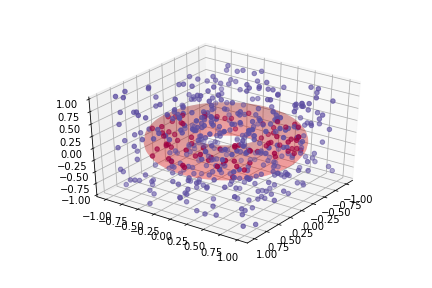
\includegraphics[width=0.7\linewidth]{donut_shape}
	\caption{Illustration of a torus in $\mathbb{R}^3$. The blue and red dots denote the two true subgroups of $X$}
\end{figure}




\subsection*{x11t2y1\_complex\_logit}
This implements the simulation settings described in \cite{xu2015regularized}. The data contains 5 binary covariates $X_1$ to$ X_5$, 5 ordinal covariates $X_6$ to $X_{10}$ and 1 continuous covariate$X_{11}$. The binary variables are generated by Bernoulli distribution with successful probability of 1/2. All ordinal covariates have 4 uniformly distribution levels. The continuous covariate is simulated form the standard normal distribution. The treatment A is independent of the covariates and takes value of 1 and 2 with equal probability. The binary response $Y$ is generated using logit as link function. The last letter in the file name corresponds to the case label in the original paper which indicates different model to generate the response Y. The detailed formulas for logit$P(Y=1)$ are described in the following:
\begin{enumerate}
	\item [A.] $0.5\cdot I_{X_3=1}+2(I_{X_2=1}+I_{X_6=3}\cdot I_{X_1=1})\cdot (2A-3)$;
	\item[D.] $\log \log (I_{X_7=3}+I_{X_8=3} +5(I_{X_6=2} + I_{X_1=1,X_2=1})\cdot(2A-3)+20)^2$;
	\item[F.] $0.5I_{X_1=1}+0.5I_{X_2=1}+2I_{X_{11}<5, X_6<2}\cdot(2A-3)$.
\end{enumerate}
The term $(2A-3)$ transforms the label of $A$ from 1/2 to -1/1.

\subsection*{x4t2y1\_discrete\_linear}
This implements the simulation settings described in \cite{su2009subgroup}. Each set contains 4 covariates $X_1$ to $X_4$ simulated from a discrete uniform distribution over (0.02, 0.04, ..., 1.00). The treatment A is independent of the covariates and takes value of 1 and 2 with equal probability. The continuous response $Y$ is generated based on different models which are described below:
\begin{enumerate}
	\item [B.] $Y=2+2\cdot (A-1) +2Z_1+2Z_2 +2\cdot (A-1)\cdot Z_1 Z_2 +\epsilon,\quad \epsilon\sim N(0,1)$;
	\item [D.] $Y=10+10\cdot (A-1)\cdot \text{exp}\{(X_1-0.5)^2+(X_2-0.5)^2\} + \epsilon, \quad \epsilon\sim N(0,1)$;
	\item [E.] $Y=2+2\cdot (A-1) +2Z_1+2Z_2 +2\cdot (A-1)\cdot Z_1 + 2\cdot (A-1)\cdot Z_2 +\epsilon,\quad \epsilon\sim Unif(-\sqrt{3},\sqrt{3})$;
	\item [F.] $Y=2+2\cdot (A-1) +2Z_1+2Z_2 +2\cdot (A-1)\cdot Z_1 + 2\cdot (A-1)\cdot Z_2 +\epsilon,\quad \epsilon\sim exp(1)$.
\end{enumerate}
The term $A-1$ transforms the label of $A$ from 1/2 to 0/1 and $Z_1=I_{X_1\le 0.5},~Z_2=I_{X_2\le 0.5}$


\subsection*{x10t2y1\_plane\_linear}
Implement the simulation setting 1 described in \cite{wang2018learning}. The dimension of $X$ is 10 and each covariate is generated from a uniform distribution $U(0,1)$. The treatment $A$ is a binary random variable coded as -1 and 1. It is randomly assigned with a probability of 0.5. The response $Y$ is generated from the following model: 
\begin{align*}
Y = 1 -2X_1 + X_2 -X_3 + 2(1-X_1-X_2)A + \epsilon_Y,
\end{align*}
where $\epsilon$ is i.i.d. $N(0,1)$.

\subsection*{x10t2y1\_circle\_linear}
Implement the simulation setting 2 described in \cite{wang2018learning}. The dimension of $X$ is 10 and each covariate is generated from a uniform distribution $U(0,1)$. The treatment $A$ is a binary random variable coded as -1 and 1. It is randomly assigned with a probability of 0.5. The response $Y$ is generated from the following model: 
\begin{align*}
Y = 1 -2X_1 + X_2 -X_3 + 8(1-X_1^2-X_2^2)A + \epsilon_Y,
\end{align*}
where $\epsilon$ is i.i.d. $N(0,1)$.


\subsection*{x4t2y1\_checkboard\_linear}
Implement the motivation example about checkboard described in \cite{zhu2015reinforcement}. The dimension of $X$ is 4 and each covariate is generated from a uniform distribution $U(0,1)$. The treatment $A$ is a binary random variable coded as -1 and 1. It is randomly assigned with a probability of 0.5. The response $Y$ is generated from the following model: 
\begin{align*}
&Y = A\times (I_{X\in D_1}-I_{X\in D_1}) , \\
&D_1 = \big\{X|\{X_1<1/3\}\cap\{ X_1>2/3\} \big\}, \\
&D_2 = \big\{X|\{X_2<1/3\} \cap \{X_2>2/3\} \big\}.
\end{align*}

\subsection*{x2t2y1\_spiral\_linear}
Implement the motivating subgroup structure of spiral shape. The dimension of $X$ is 2 and each covariate is generated from a uniform distribution $U(0,1)$. The treatment $A$ is a binary random variable coded as -1 and 1. It is randomly assigned with a probability of 0.5.
Denote $tan(\theta) = \frac{X_2}{X_1}$ and $r = \sqrt{X_1^2+X_2^2}$.
The response $Y$ is generated from the following model: 
\begin{align*}
&Y = A\times (I_{X\in D_1}-I_{X\in D_1}) , \\
&D_1 = \big\{X|0.1\leq r - 1.5(\theta+(2k+0.5)\pi)\leq 2,\;k=0,1,2 \big\}, \\
&D_2 = \big\{X|0.1\leq r - 1.5(\theta+(2k+1.5)\pi)\leq 2,\;k=0,1,2 \big\}.
\end{align*}
The spiral shape is illustrated below:
\vspace{-5mm}
\begin{figure}[h]
	\centering
	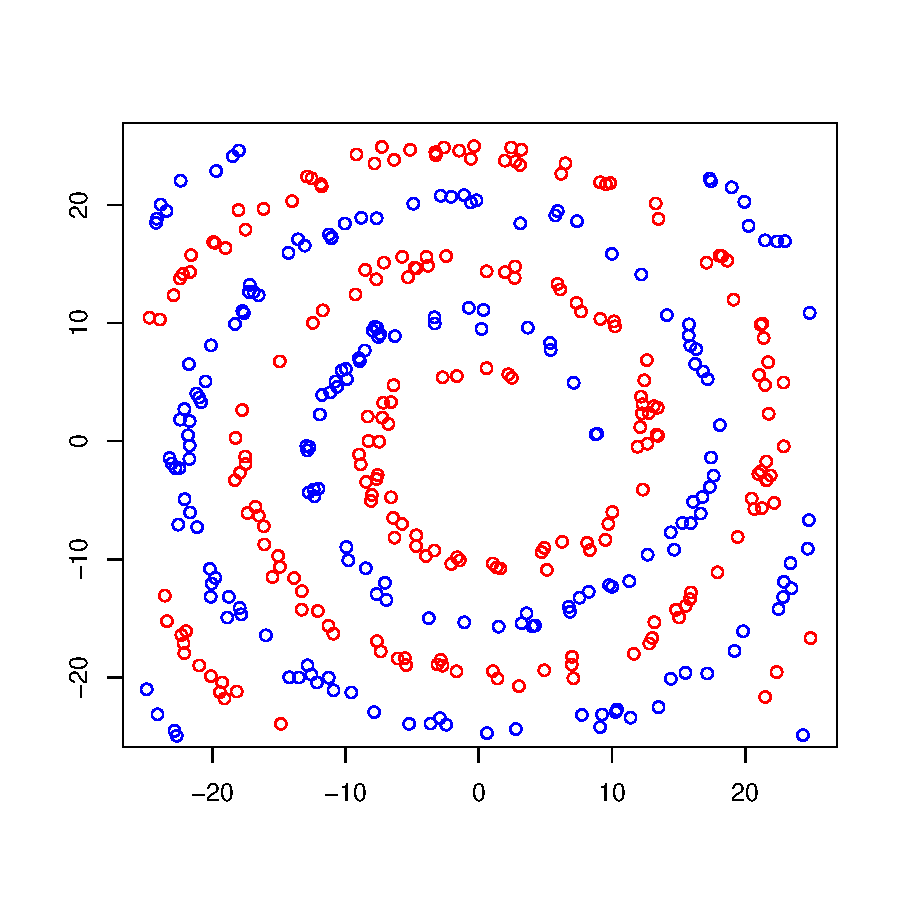
\includegraphics[width=0.5\linewidth]{spiral}
	\vspace{-5mm}
	\caption{Illustration of the spiral subgroup. The blue color and red color represent two subgroups}
	\label{fig:spiral}
\end{figure}



\subsection*{x10t2y1\_cox\_circle}
Implement the Cox model with circle subgroup structure. The dimension of $X$ is 10 and each covariate is generated from a uniform distribution $U(0,1)$. The dimension of truly associated covariates is 4. The treatment $A$ is a binary random variable coded as -1 and 1. It is randomly assigned with a probability of 0.5. The survival time $T$ is generated as following: we set the constant baseline hazard as 1.
$$T \sim \exp(1 -2X_1 + X_2 -X_3 + 8(1-X_1^2-X_2^2)A )$$

\subsection*{x1t8y3\_Q\_survival}
Implement a simplified version of the simulation setting described in \cite{goldberg2012q}. We use the original notation for convenience. Denote the discrete time point $i=0,1,2,3$, the tumor size at time $i$ as $T(i) \in [0,1]$ and the wellness at time $i$ as $W(i)\in [0.25,1]$. The trial begin with $T(0)=1$ and $W(0)$ uniformly distributed on [0.5,1]. At each time point $i$, we consider two optional treatments A and B. The immediate effects of A are:
\begin{eqnarray}
W(i^+|A)&=&W(i)-0.5,\\
T(i^+|A)&=&T(i)/(8W(i)),
\end{eqnarray}
where $W(i^+|A)$ is the wellness at $i$ after treatment A. Similarly the immediate effects of the treatment B are:
\begin{eqnarray}
W(i^+|B)&=&W(i)-0.25,\\
T(i^+|B)&=&T(i)/(4W(i)).
\end{eqnarray}
The wellness and the tumor size of the next time point are computed as:
\begin{eqnarray}
W(i+1)&=&\max(~W(i^+)+(1-W(i^+))(1-2^{-1/2})+\epsilon,0.25~),\\
T(i+1)&=&\min(~T(i^+)+4T(i^+)/3+\epsilon,1~),
\end{eqnarray}
where $\epsilon \sim N(0,0.1)$
For $i=0,1,2$, two treatments are assigned to the patient with equal probability independently. We use $A_1A_2A_3$ to denotes the treatment sequence where $A_i\in {A,B}$. We encode all the eight probable treatments into $1,2,..8$, i.e., $1=AAA,~2=AAB,~3=ABA,~4=BAA,~5=ABB,~6=BBA,~7=BAB,~8=BBB$. So the action is eight dimensional. Besides, we define one dimensional $X=W(0)$. We also assume the survival function of the patient as an exponential distribution with mean $S(i)=3(W(i^+)+2)/(20T(i^+)),~ i=0,1,2$. We define three dimensional $Y=[S(0)~S(1)~S(2)]$ and the optimal action is chosen to maximize $\sum_{i=0}^2 S(i)$.


\bibliographystyle{chicago}
\bibliography{ref_simulation}


\newpage

\begin{table}[htbp]
  \centering
  \caption{\emph{An illustration training dataset}}
    \begin{tabular}{c|c|c|cccc}
    \hline
    \hline
    ID & $Y$     & $A$   & $X_1$    & $X_2$    & $X_3$    & $\cdots$ \\
    \hline
    1&1.5  & 1     & 0     & 26    & 7.8   & $\cdots$ \\
    2&1.2  & 2     & 1     & 28    & 8.2   & $\cdots$  \\
    3&0.3  & 3     & 1     & 31    & 8.9   & $\cdots$  \\
    4&0.9  & 2     & 0     & 35    & 9.4   & $\cdots$  \\
    5&1.7  & 1     & 1     & 22    & 7.3   & $\cdots$  \\
    $\vdots$ & $\vdots$    & $\vdots$    & $\vdots$   & $\vdots$     & $\vdots$     & $\ddots$  \\
    n & 1.6 & 2 & 0 & 29 & 8.1 & $\cdots$ \\
    \hline
    \hline
    \end{tabular}%
  \label{tab:TrainingDataExample}%
\end{table}%

\begin{table}[htbp]
  \centering
  \caption{\emph{An illustration testing dataset: nnn\_xxxx\_Testing\_1.csv.} }
    \begin{tabular}{c|cccc}
    \hline
    \hline
    ID &  $X_1$    & $X_2$    & $X_3$    & $\cdots$ \\
    \hline
    1& 0     & 26    & 7.8   & $\cdots$ \\
    2& 1     & 28    & 8.2   & $\cdots$  \\
    3& 1     & 31    & 8.9   & $\cdots$  \\
    4& 0     & 35    & 9.4   & $\cdots$  \\
    5& 1     & 22    & 7.3   & $\cdots$  \\
    $\vdots$ &  $\vdots$   & $\vdots$     & $\vdots$     & $\ddots$  \\
    N &  0 & 29 & 8.1 & $\cdots$ \\
    \hline
    \hline
    \end{tabular}%
  \label{tab:TestingDataExample1}%
\end{table}


\begin{table}[htbp]
  \centering
  \caption{\emph{An illustration testing dataset: nnn\_xxxx\_Testing\_2.csv.} $Y(a)$ is the potential outcome taking treatment $a$, $A$ is the observed treatment assignment, and $A^o$ is the oracle optimal treatment assignment based on $d(X,A)$.}
    \begin{tabular}{c|cccc|cc}
    \hline
    \hline
    ID &  $Y(1)$    & $Y(2)$    & $\cdots$  & $Y(k)$ & $A$ & $A^o$   \\
    \hline
    1& 1.2    & 1.5    &  $\cdots$  & 1.3 & 3 & 2 \\
    2& 1.3    & 1.1    &  $\cdots$  & 1.4 & 2 & 3 \\
    3& 0.9    & 0.8    &  $\cdots$  & 1.7 & 1 & 3 \\
    4& 1.8    & 1.6    &  $\cdots$  & 1.2 & 1 & 1 \\
    5& 1.4    & 1.4    &  $\cdots$  & 1.5 & 2 & 2 \\
    $\vdots$ &  $\vdots$   & $\vdots$     & $\ddots$     & $\vdots$ &  $\vdots$   & $\vdots$ \\
    N & 1.7    & 1.4    &  $\cdots$  & 1.1 & 3 & 1 \\
    \hline
    \hline
    \end{tabular}%
  \label{tab:TestingDataExample2}%
\end{table}

\begin{table}[htbp]
	\centering
	\caption{\emph{An illustration testing dataset: nnn\_xxxx\_Testing\_2.csv.} The observed benefit is $V=1/N \sum (1.2+1.1+0.9+1.6+1.4+\cdots+1.4)$, and theoretical optimal value is $V^o=1/N \sum (1.5+1.3+0.8+1.8+1.4+\cdots+1.7)$, and the estimated value is $\hat{V}=1/N \sum (1.5+1.3+0.9+1.6+1.4+\cdots+1.7)$.}
	\begin{tabular}{c|cc|ccc}
		\hline
		ID &  $Y(1)$    & $Y(2)$    & $A$ & $A^o$ & $\hat{A} $  \\
		\hline
		1& 1.2    & 1.5    &   1& 2 &2 \\
		2& 1.3    & 1.1    &  2 & 1 &1\\
		3& 0.9    & 0.8    &    1 & 2 &1 \\
		4& 1.8    & 1.6    &   2 & 1 &2 \\
		5& 1.4    & 1.4    &  2 & 2 &2 \\
		$\vdots$ &  $\vdots$   & $\vdots$     & $\vdots$     & $\vdots$ &  $\vdots$    \\
		N & 1.7    & 1.4    &   2 & 1 &1\\
		\hline
		\hline
	\end{tabular}%
	\label{tab:TestingDataExample3}%
\end{table}


\end{document}}

